\begin{refsection}


\chapter{Introduction}
The fusion energy has been a goal of active pursuit for nearly seventy years.
The core problem for fusion energy development, as compared to fusion based
weaponry, is the problem of confinement. While the sun had successfully
achieved net positive fusion energy through the successful application
gravitational confinement, that approach is unfortunately not practical for
Earth based application. Instead, a wide variety of alternative confinement
strategies have been attempted, broadly separated into magnetic confinement and
inertial confinement. Where as the inertial confinement focuses on short,
repeated pulses of fusion reaction at very high densities driven by enormous
lasers, magnetic confinement focus on using the magnetic field to restrict the
movement of plasma particles long enough to produce net fusion power. Magnetic
confinement fusion has been favored by the majority of the fusion community, in
part because it does not involve high frequency explosions. magnetic
confinement fusion further divides into a number of 'concepts' based on the
magnetic topology used, with the TOKAMAK taking the lead in achieved plasma
temperature and duration. Everything else is commonly refereed to as
'alternative concepts', and this work deals with one of them: the Reversed
Field Pinch (RFP). In particular, confinement, transport, and heating
characteristics of ions in the RFP.


\section{The Reversed Field Pinch and its history}

\begin{figure}[!htb]
	\centering
	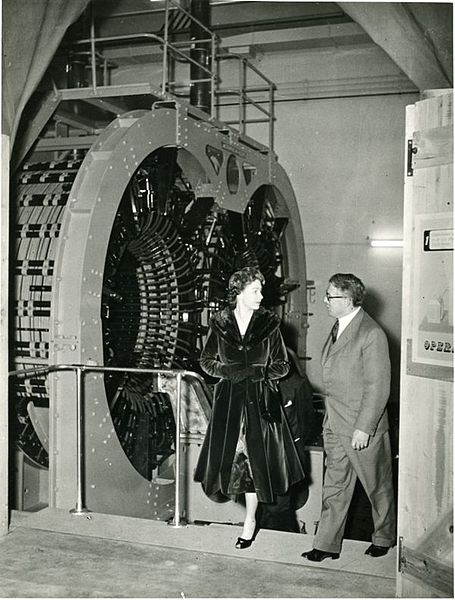
\includegraphics[width = 0.75\linewidth]{./1_Introduction/queen_at_zeta.jpg}
    \label{fig:Queen_at_ZETA}
    \caption[Queen Elizabeth II at the ZETA experiment]{Queen Elizabeth II of Canada and assorted other places, vising ZETA during it's construction in 1957. Photograph by UKAEA}
\end{figure}%

The story of the RFP starts with the Zero Energy Thermonuclear Assembly (ZETA).
Initially built as an extension of the now abandoned toroidal pinch confinement
concept, ZETA was one of the leading fusion experiment of its time, often know
for making and later retracting the first claim of observation of fusion
neutrons, for a time galvanizing world interesting in the imminent arrival of
unlimited energy via fusion. Alas, the claim was made in haste. But persistence
and hard work eventually let scientists at ZETA to discover the spontaneous
reversal of the magnetic field associated with the most stable (quiescent)
period of ZETA's plasmas \cite{Butt_IAEA66,Robinson_IAEA69}. This phenomenon
was explained by J. Taylor in 1974 as a naturally result from the relaxation of
the magnetic topology towards lower energy state \cite{Taylor74}. These were
the foundational documents of the RFP.

\begin{align}\label{eqn:helicity}
	K \equiv \int_{V} \vec{A} \cdot \vec{B} d\tau
\end{align}

Specifically, Taylor posited that in a toroidal plasma of finite resistivity
constrained by a perfectly conducting shell, the magnetic helicity $K$ is
conserved (eqn. \ref{eqn:helicity}). With this constraint, the plasma relaxes
toward a state of minimum magnetic energy characterized by eqn.
\ref{eqn:min_energy_condition}, where $\mu \varpropto K/ \Psi ^2$, is a
constant unrelated to permeability . 

\begin{align}\label{eqn:min_energy_condition}
    \nabla \times \vec{B} = \mu \vec{B}
\end{align}

In cylindrical approximation, the solution to equation
\ref{eqn:min_energy_condition} are Bessel functions (eqn.
\ref{eqn:rfp_solution}) where $B_Z$ reverses in the edge if the plasma current
is high compared to toroidal flux \cite{Taylor74}.

\begin{align}\label{eqn:rfp_solution}
B_z &= B_0J_0(\mu r)\\
B_\theta &= B_0 J_1(\mu r)\\
B_r & = 0
\end{align}

The magnetic topology of atypical RFP is shown in figure
\ref{fig:RFP_geometry}. The relatively low $B_t$ means the RFP have several
advantages over the Tokamak. In the tokamaks, powerful toroidal field coils (TF
coils) are used to generate toroidal flux and keep the safety factor q is kept
above 1 in order to stabilize the plasma. This leads to limits on the toroidal
plasma current depending on the the available coil generated toroidal flux.
This in turns is limited by engineering constrains in terms of magnetic coil
construction. The reversed field pinch avoids these constrains, and
consequently can be constructed with much simpler and cheaper TF coil
arrangements, as well as being more easily reach very high current levels to
take advantage of large Ohmic heating, possibly to ignition levels.

\begin{figure}[!htb]
	\centering
	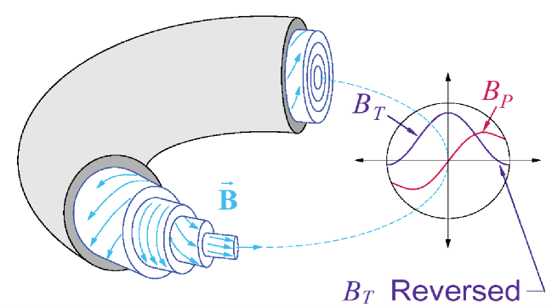
\includegraphics[width = 1.\linewidth]{./1_Introduction/RFP_mag_geometry.png}
	\label{fig:RFP_geometry}
	\caption[RFP magnetic topology]{Illustration of the RFP topology. The most distinct features of the RFP is the similar magnitudes of $B_t$ vs. $B_p$, as well as the fact that $B_p$ reverses direction near the edge.}
\end{figure}%

However, the magnetic topology also poses challenges to the RFP's confinement
characteristics. Taylor noted that the relaxation of the magnetic field is made
possible by the finite resistivity, but did not speculate on the 'method' of
relaxation. Experiments have shown that the relaxation occurs via resistive
tearing mode instabilities which poses a challenge to RFP confinement
characteristics.

\begin{figure}
	\centering
    \label{fig:q_profile}
    
    \caption[Example RPF q profile]{q profile typical of the plasmas studies in this work. Note the closely space resonant surfaces.}

\end{figure}

\section{Tearing modes, it's suppression via PPCD, and improved confinement}
\begin{figure}[!htb]
	\centering
	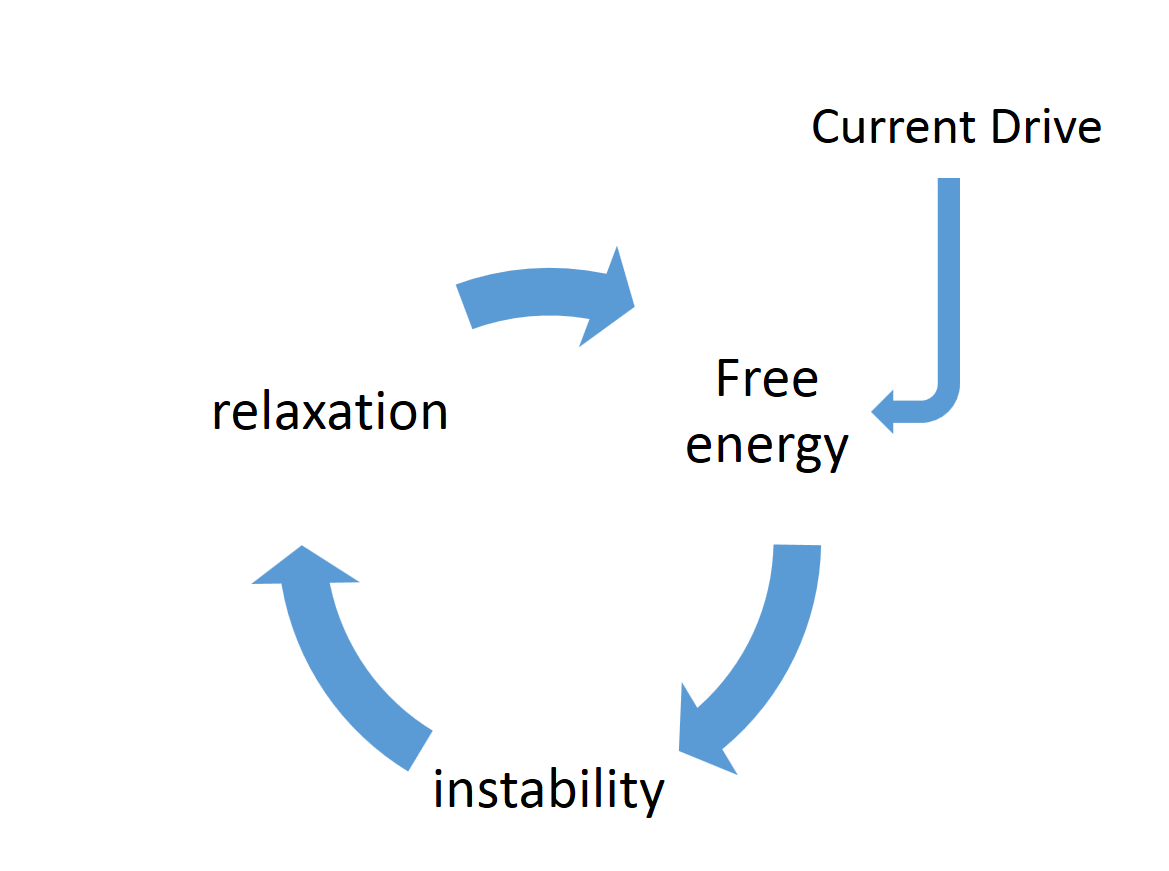
\includegraphics[width = .6\linewidth]{./1_Introduction/the_sawtooth_cycle.PNG}
	\label{fig:sawtooth_cycle}
	\caption[The sawtooth cycle]{The sawtooth cycle that dominates standard RFP plasmas. Improving RFP confinement involves the suppression of this cycle. The PPCD approach involves the suppression of the tearing mode instabilities while inductively driving the plasma current profile relaxation.}
\end{figure}%

The finite resistivity of the plasma allows for the reconnection of the
magnetic field lines and the formation of magnetic islands through tearing mode
instabilities. Tearing modes are unstable at magnetic resonant surfaces where
the safety factor $q \equiv \frac{rB_T}{R_0B_p}$ is a rational number, ie $q =
\frac{m}{n}$ where m and n are integers. The location of these unstable regions
form 'resonant' surfaces that are typically labeled by their m and n numbers.
The RFP have q significantly lower than 1 everywhere, and further decreases
monotonously towards the edge where it will cross 0. An example q profile is
show in figure \ref{fig:q_profile}. This leads to the existence of a large
number of resonant surfaces, especially close to the reversal surface. 

These closely spaced resonant surfaces and the tearing mode instabilities that
they 'host' creates regions of overlapping magnetic islands that turns the
magnetic field stochastic, greatly reducing the confinement characteristics.
Further, the tearing modes in standard RFP enables the violent relaxations
events know as the sawtooth crashes, where the accumulation of free energy in
the form of parallel current ($J_{\parallel}$) gradient will cause a sudden
increase of magnetic reconnection and tearing mode fluctuation. This process
then repeats as the parallel current gradient builds up again in what is know
as the sawtooth cycle (fig \ref{fig:sawtooth_cycle}). Though ion heating is
observed with the sawtooth
crashes\cite{Bodin1980Reversed-field-pinchReserarch}, they greatly disrupts
confinement of particles and limit the RFP's viability as a fusion concept.

\begin{figure}[!htb]
	\centering
	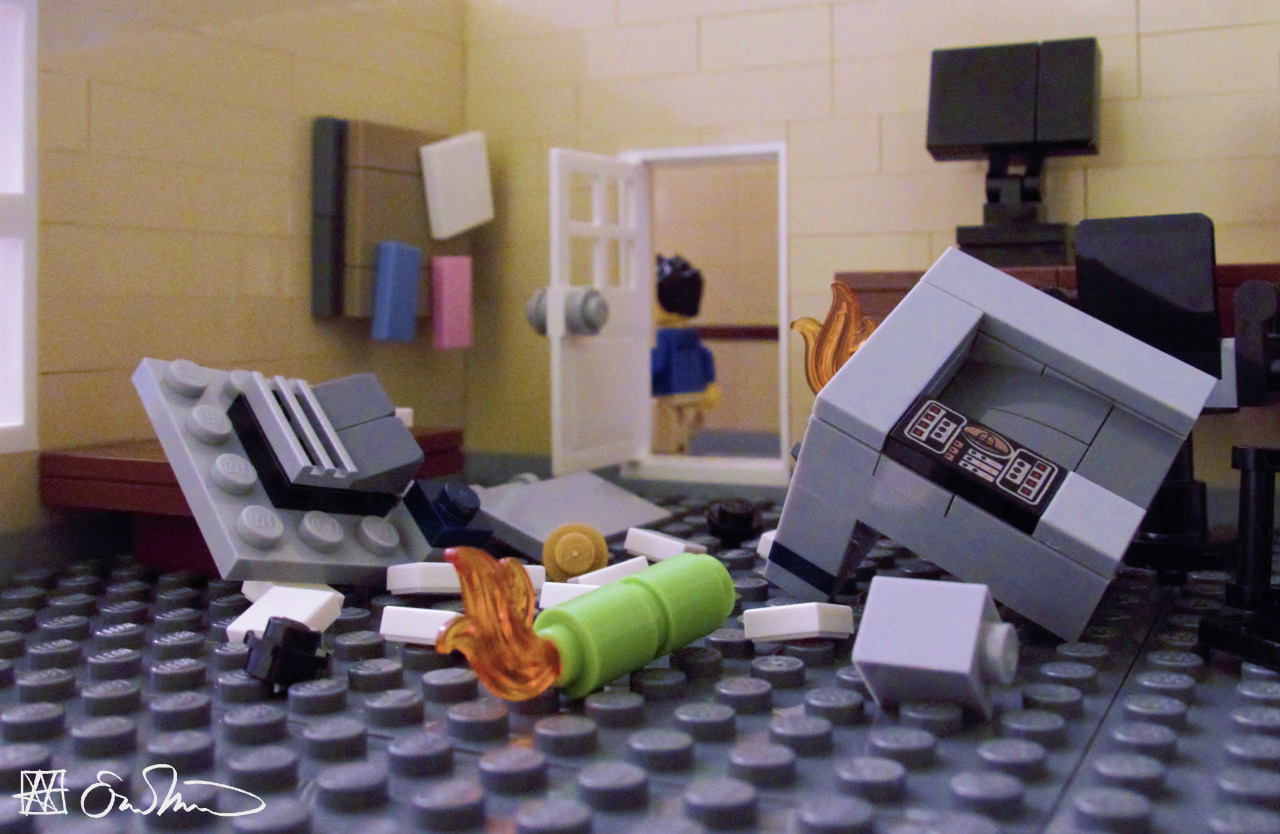
\includegraphics[width = .8\linewidth]{./1_Introduction/violent_relaxation.jpg}
	\label{fig:violet_relaxation}
	\caption[An illustration of violent relaxation]{An artist's impression of a violent relaxation event. By the Lego Grad Student}
\end{figure}%

One very successful way of reducing tearing mode activity and its detrimental
effects on confinement is through the control of $J_{\parallel}$ profile,
thereby reducing the available free energy from it's gradient at the resonant
surfaces\cite{Sarff1995TransportPinch}. On MST, this is done inductively
through a process called Pulsed Parallel Current Drive (PPCD). PPCD drives
parallel currently near the reversal surface (details discussed in section
\ref{sec:MST}), essentially aiding the plasma in reaching itspreferred' state
of with a flat $J_{\parallel}$ profile so it doesn't 'have to' through 'the use
of' sawtooth crashes. Further refinements of this process is also able to
reduce the residual, m = 0 related, magnetic reconnection, achieving
significantly improved confinement for $\geq 10ms$ \cite{Chapman2001}.



\section{Characteristics of PPCD plasma}

PPCD reduces the tearing mode fluctuation levels significantly as shown in
figure \ref{fig:ppcd_fluc}


It is well known that magnetic reconnection such as sawtooth are bad, but are
they cruel? It's a question that have yet to answered in all these years. How
do sawtooth events stack up again the terrible events perpetrated by powerful
men through the ages such as war and famine and worse things. We don't really
know.



They are pretty to look at and stuff. Also Jim Reynolds predicted pinch. Also
significant reduction in fluctuation. Also $T_e$ increase and hot, and have
bursts occasionally, also transport transport transport also stochasticity
decreases, also transient, and some other stuff.


[[Both Santhosh's observation of classical transport but also Reynold's prediction]]


\section{m = 0 bursts in EC and PPCD plasmas}

Bill Young looked at the m = 0 in EC plasmas because he can't look at sawtooth.
Ring like structure, and what not. Also D. Adams made a post for it, measuring
the ring structure, looks good.


[[Bill Young's stuff will be here, as well whatever he cites.]]


\section{What this thesis is all about}
[[Signposting is important]]



Ion transport is important area of research for several reasons in the context
of fusion confinement geometry. The most basic being that it is ion temperature
that is relevant to the rate of fusion reactions. But in particular, there is
long standing disagreement in the field regarding the mechanism behind the well
known anomalous ion heating associated with sawtooth events. At the same time,
there has been confusion about the existence and magnitude of anomalous heating
during periods of improved confinement achieved through parallel current drive.

The RFP geometry suffers from regular global sawtooth events associated with
tearing mode reconnections. While the violent magnetic fluctuations [[Draw
connections with solar and dynamo stuff]]

[Now draw connections with fusion, confinement and whatnot]
\printbibliography%[title={Section bibliography}]

\end{refsection}
